\chapter{Aufgabe}
\section*{a}
\subsection*{i}
Siehe Abbildung \ref{fig:graphLCOM}

\begin{figure}[h!]
	\centering
	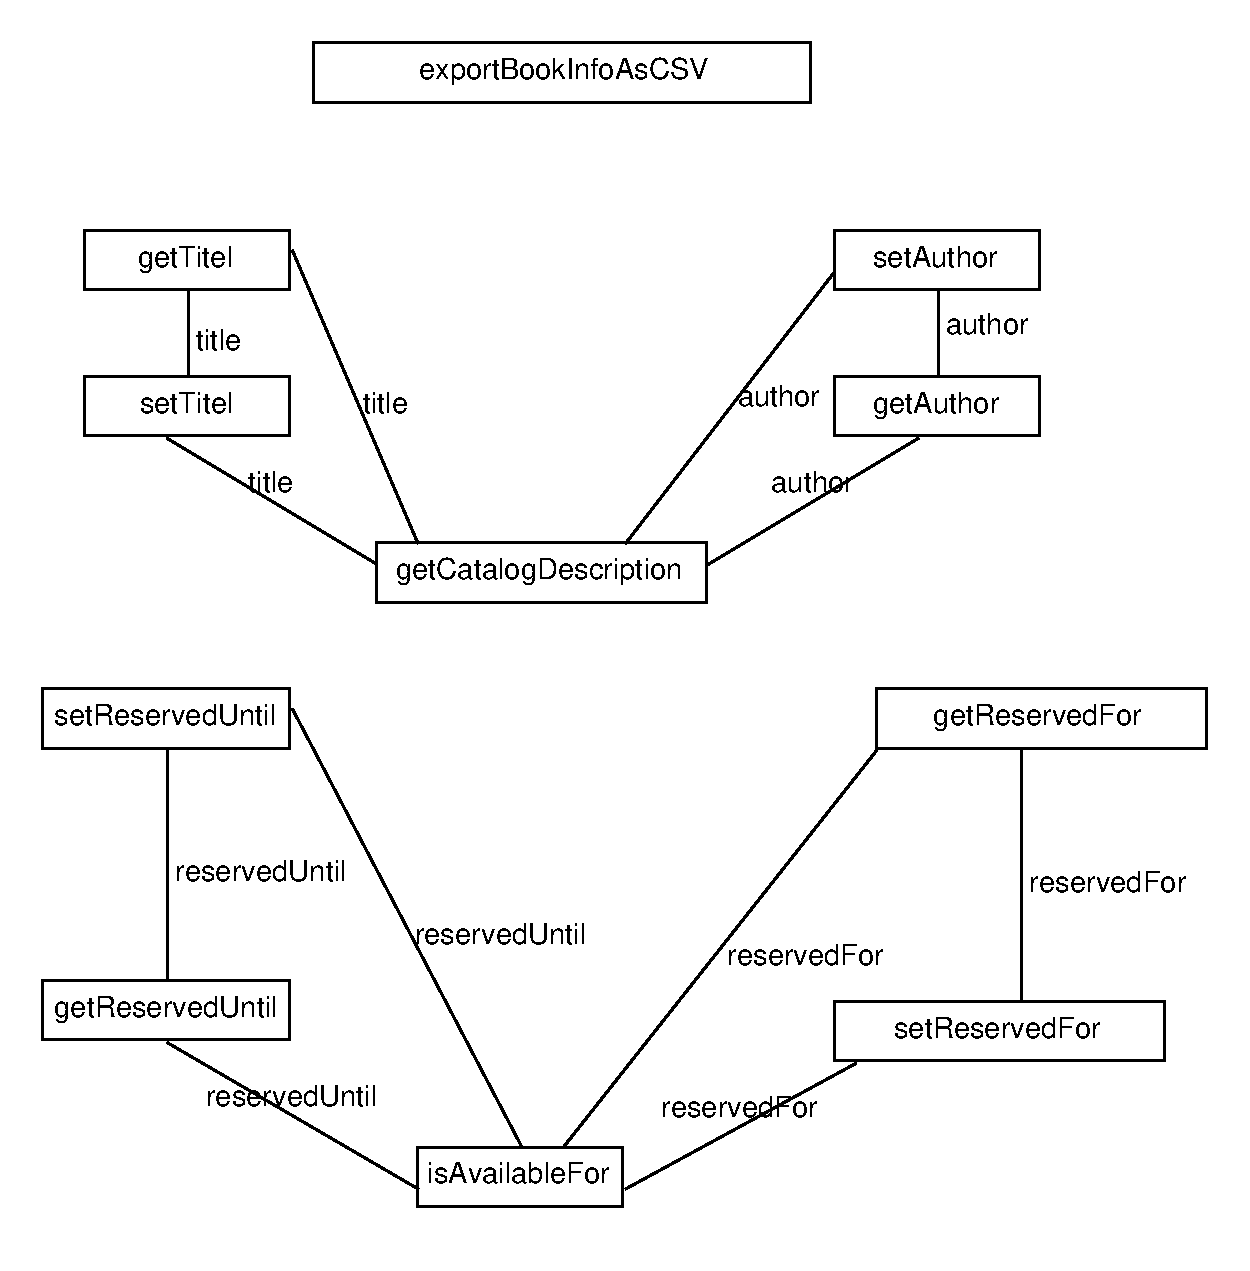
\includegraphics[width=0.8\textwidth, clip]{images/graphLCOM.pdf}
	\caption{Zusammenhangsgraph der Klasse Book für das  LCOM Verfahren. }
	\label{fig:graphLCOM}
\end{figure}
\subsection*{ii}
\textbf{LCOM = 3 von 11}



\section*{b}
Bei erstem Betrachten der Implementation erschien deren Kohäsion nicht optimal zu sein. Drei nicht zusammenfallende Verantwortungen sind alle in einer Klasse enthalten, die noch dazu ein sehr allgemeines Konzept beschreibt, was eine hohe Kohäsion sehr wünschenswert machen würde.\\
Der berechnete Wert spiegelt dies gut wieder, da er mit 3 auf jeden Fall nicht optimal ist. Angesichts der hohen Methodenanzahl in der Klasse hätte er aber dem Empfinden nach noch höher ausfallen können.
Die Verantwortungen der Klasse \texttt{Book} sind:
\begin{enumerate}
	\item Verwaltung der Daten eines einzelnen Buches
	\item Verwaltung der Daten Bezüglich der Ausleihe eines einzelnen Buches
	\item Exportieren der Daten eines einzelnen Buches als csv-Datei
\end{enumerate}
 Der ermittelte \textbf{LCOM}- Wert deckt sich also hier genau mit der Anzahl der Verantwortungen der Klasse.
 
 
\section*{c}
\section*{d} 